\section{Rozpoznávanie tváre}
Rozpoznávanie tváre je jedným z úkonov, ktoré človek robí pravidelne a bez námahy v každodennom živote.
Široká dostupnosť silných počítačov za nízku cenu vytvára obrovský záujem o automatické spracovanie digitálneho
obrazu v širokom spektre aplikácií, ako sú napríklad biometrická autentifikácia, monitorovanie osôb,
interakcia s počítačom či spravovanie multimédií.
Výskum a vývoj v oblasti rozpoznávania tvárí nasleduje tento trend
automaticky.\\
\indent Hlavnými výhodami využívania rozpoznávania tvárí voči iným biometrickým metódam ako napríklad odtlačky prstov či dúhovka,
je ich prirodnené a nerušivé používanie, ale najmä možnosť použitia na vačšiu vzdialenosť. Zo šiestich biometrických metód (tvár, odtlačky prstov, dlaň, hlas, dúhovka, podpis)
je podľa The International Civil Aviation Organization(ICAO)\cite{icao} rozpoznávanie tváre primárnou metódou pri kontrole identity na letisku.\\
\indent Prvým automatickým systémov na rozpoznávanie tvárí bol podľa\cite{handbookface}, systém navrhnutý Takeo Kanadem v jeho práci\cite{kanade1974} z roku 1974.
Za ním nasledovalo obdobie bez výraznejšieho pokroku v automatickom rozpoznávaní tváre, až do roku 1990, kedy Sirovich a Kirby zverejnili článok\cite{kirby1990application},
v ktorom popisujú využitie nizko dimenzionálnych reprezentácií tváre odvodenej z Karhunen-Loevovej transformácie alebo Principal Component Analysis(PCA).
Podľa Jaina v\cite{handbookface} bol ďalším veľkým míľnikom práca\cite{turk1991eigenfaces} od Turka a Pentlanda na vlastných vektorov tváre (eigenface),
ktorá znovu naštartovala výskum v oblasti rozpoznávania tváre. Medzi ďalšie míľniky tiež Jain zaraďuje prácu na Fisherovej metódae\cite{belhumeur1997eigenfaces},
ktorá aplikuje Linear Discriminant Analysis(LDA) po aplikovaní PCA k dosiahnutiu vyššej presnosti, výskum na lokálnych Gaborových filtroch\cite{wiskott1997face}
k dosiahnutiu efektívnejších príznakov tváre a prístup AdaBoost učenia, založeného na architektúra kaskádneho klasifikátora pre detekciu v reálnom čase\cite{viola2001rapid}.\\
\indent Od obdobia kedy bola narhnutá Eigenface metóda nastal veľký pokrok v oblasti rozpoznávania tváre.
V kontrolovaných podmienkach, kde je možné ovládať svetelnosť,
postoj osoby či výraz tváre, prekonáva automatické rozpoznávania tváre ľudí, a to najmä pokiaľ databáza obsahuje veľké množstvo snímkov tváre.
Napriek tomu rozpoznávanie tváre
stále čelí mnohým výzvam, najmä problematike rozpoznávania tváre v neriadených podmienkach.

\subsection{Rozdelenie}
Ako aj ostatné biometrické systémy, aj rozpoznávanie tváre funguje v jednom alebo oboch z režimov:
\begin{itemize}
    \item Verifikácia (autentifikácia)
    \item Identifikácia tváre
\end{itemize}

Pri verifikácii tváre ide o porovnanie jedna k jednej, čo znamená, že jeden snímok tváre sa porovnáva len jedným záznamom identity v databáze, za ktorú sa prehlasuje.
Typickým využitím tohoto režimu je samoobslužná kontrola identity prostredníctvom elektronického pasu\cite{handbookface}.\\
\indent Identifikácia tváre zahŕňa porovnanie jedna k mnohým, čo znamená, že jeden snímok tváre sa porovnáva s viacerými záznamami identít v databáze a vyberie jednu\cite{handbookface}.
V niektorých prípadoch využitia je postačujúce nájsť len najpodobnejšiu identitu.
V iných prípadoch, ako napríklad sledovanie podozrivých osôb,
je okrem nájdenia najpodobnejšej tváre potrebné zaviesť aj prah spoľahlivosti, a tie tváre ktoré dosiahli mieru podobnosti väčšiu ako je prah, sú zaznamenané.\\
\indent Úspešnosť systému na rozpoznávanie tváre závisí vo veľkej miere na množstve variabilných faktorov, ako je osvetlenie, poloha tváre, mimika, vek, make-up, účes,
brada či pohyb tváre. Na základe týchto faktorov Jain rozdeľuje\cite{hanbookface} na 2 kategórie vzhľadom na miery spolupráce užívateľov:

\begin{itemize}
    \item Scenár so spolupracujúcim užívateľom
    \item Scenár s nespolupracujúcim užívateľom
\end{itemize}

\indent Prípad spolupracujúceho užívateľa je využívaný napríklad pri prihlasovaní do počítača, riadenie fyzického prístupu, elektronické pasy (e-passport), teda prípady kedy má
užívateľ záujem spolupracovať na správnom zoznímaní tváre (napr. pod správnym zoznímaním tváre môžeme rozumieť napríklad snímok tváre z predu s neutrálnym výrazom a otvorenými očami)
kvôli prístupu alebo povoleniu.\\
\indent V prípade nespolupracujúceho užívateľa, ktorý je typické pre už spomínané sledovanie podozrivých, si osoba nie je vedomá toho, že podlieha identifikácii.
Čo sa týka vzdialenosti
medzi tvárou osoby a kamerou, sa v spolupracujúcom scenári využíva krátka vzdialenosť, typicky o jedného metra, a ide teda o oveľa jednoduchšiu úlohu v porovnaní s identifikáciou
nespolupracujúcej osoby často na väčšiu vzdialenosť.

\subsection{Proces identifikácie}
Jain popisuje rozpoznávanie tváre takto: ``Rozpoznávanie tváre sa zaraďuje medzi problémi rozpoznávania vzorov, kde tvár, ktorá je reprezentovaná ako trojzormerný objekt,
podlieha odlišnostiam vo svetle, postoji, výraze a iných faktoroch, potrebuje byt identifikovaná na zákle zozbieraných obrázkov``\cite{handbookface}.
Zatiaľ čo roznávanie tváre z dvojrozmerného snímku je dnes bežne používané vo vačšine prípadov, v niektorých, najmä tých ktoré vyžadujú vyššiu bezpečnosť,
sa využíva trojrozmerný snímok tváre,
prípadne snímky tváre mimo bežne viditeľného spektra - napr. termografický snímok tváre.  Systém na rozpoznávanie tváre sa podľa Jaina\cite{handbookface} vo všeobecnosti skladá zo štyroch
základných častí, ako je ukázané na obrázku\ref{fig:workflow}:
\begin{itemize}
    \item Detekcia tváre a lokalizácia bodov tváre
    \item Normalizácia tváre
    \item Extrakcia príznakov
    \item Hľadanie zhody tváre
\end{itemize}

\begin{figure}[H]
    \centering
    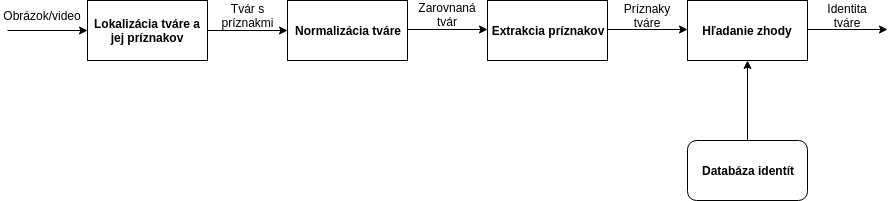
\includegraphics[width=1\linewidth]{img/workflow}
    \caption{Proces rozpoznávania tváre}
    \label{fig:workflow}
\end{figure}

\indent  Pri detekcií tváre ide primárne o oddelenie oblasti tváre od pozadia snímku.
V prípade videa je potrebné sledovať (track) detekovanú tvár naprieč niekoľkými snímkami videa pomocou komponentu na sledovanie pohybu tváre.
Zatiaľ čo detekcia tváre poskytuje len hruby odhad polohy a veľkosti tváre, lokalizácia bodov tváre najde už konkrétne časti tváre,
ako sú napríklad oči, nos, obrys tváre a podobne.
Lokalizácia bodov tváre je zväčša vykonanávaná osobitným komponentom na lokalizáciu bodov alebo komponentom na vyrovnanie (alignment) tváre.\cite{handbookface}\\
Normalizácia tváre ide o normalizáciu tváre v geometrickom a fotometrickom zmysle.
Tento krok je nevyhnutný, pretože sa od najnovších a najlepších (state-of-the-art) rozpoznávacích metód očakáva, že dokážu rozpoznať tvár v rôznych polohách a rôznom svetle.
Geometrická normalizácia vykonáva transformáciu tváre do štandartného formátu snímku pomocou orezania (crop) tváre.
Snímok je následne zakrivený (warp) a upravený (morph) kvôli ešte lepšej a presnejšej normalizácií tváre.
Úlohou fotometrickej normalizácie je spracovanie snímku na základe osvetlenie či farebnej škály.\cite{handbookface}\\
\indent Extrakcia príznakov je vykonávaná na normalizovanom snímku tváre, s cieľom vybrať charakteristické infomácie, ktoré sú užitočné pri rozlišovaní tvárí rozdielnych osôb,
pričom odolný voči odchýlkam v geometrickej a fotometrickej normalizácii.
Extrahované príznaky sú nasledne použité pri hľadaní zhody s identitou.\cite{handbookface}\\
\indent Pri hľadaní zhody tváre sa porovnávajú extrahované priznaky zo vstupnej tváre s jednou alebo viacerými tvárami ktoré už sú zapísané v databáze.
Výsledkom porovnania s jednou tvárou je výsledkom odpoveď áno alebo nie (verifikácia).
V prípade porovnávania s viacerými tvárami je výsledkom indetita vstupnej tváre, za predpokladu, že identita ktorá je nájdená presiahne prah spoľahlivosti,
inak vráti informáciu, že tvár je neznáma.
V súčastnosti je v tejto oblasti najväčšou výzvou nájsť spoľahlivé meranie vhodné na určenie podobnosti príznakov tváre.\cite{handbookface}\\
\indent Presnosť systému na rozoznávanie tváre vo veľkom závisí na správnosti extrahovaných príznakoch tváre, ktoré naopak, závisia od správnej lokalizácii a normalizácii tváre.

\subsection{Techniky rozpoznávania tvári}
Zhao rozdeľuje\cite{zhao2003face} algoritmy rozponávania do dvoch základných kategórií, vzhľadom na spôsob extrakcie príznakov:
\begin{itemize}
    \item Metódy založené na príznakoch (feature-based)
    \item Medódy založené na vzhľade (appearance-based)
\end{itemize}

Metódy založené na príznakoch využívajú rôzne vlastnosti a geometrické atribúty na popis tváre, ako sú napríklad vzdialenosti či uhly medzi bodmi tváre.
Na druhej strane, metódy založené na vhľade využívajú globálne vlastnosti tvárového vzoru.
Typickou črtou algoritmov založených na vhľade je výpočet bázových vektorov, na ktoré je následne tvár premietnutá.
Koeficienty takejto projekcie sú potom použité k efektívnej reprezentácii údajov tváre\cite{handbookbio}.
Obľúbené algoritmy ako sú Principal Component Analysis (PCA), Linear Discriminant Analysis (LDA), Indenpendent Component Analysis (ICA),
Local Feature Analysis (LFA), Manifolds, Correlation Filters alebo Tensorfaces sú založené práve na vhľade tváre.
Holistický prístup k rozpoznávaniu tváre má však často problémy pri rôznych polohách tváre\cite{handbookbio}.

\subsubsection{Eigenfaces (PCA)}
Podstatou metódy Eigenfaces navrhnutej Turkom a Pentlandom\cite{turk1991eigenfaces}, tiež známej ako PCA,
je hľadanie najmenšej kvadratickej chyby lineárneho podpriestoru,
ktorý mapuje dáta z originálneho N-rozmerného priestoru na M-rozmerný priestor príznakov, kde M << N .
Týmto dosiahneme redukciu dát do M rozmeného priestoru využitím M vlastných vektorov matice kovariance, ktoré korešpondujú s najväčšími hodnotami vlastných čísel\cite{handbookbio}.
Konečné bázové vektory ktoré sú najvhodnejšie na popis dát, sú nájdené pri procese optimalizácie, ktorej podstatou je  maximalizácia variancie premietnutých dát.
Jain popisuje\cite{handbookbio} proces výberu bázových PCA vektorov W optimalizačnou funkciou\eqref{eqn:pca}, kde S\textsubscript{T} označuje úplne maticu rozptylu,
ktorá obsahuje kovariancie dát tváre.


\begin{equation}\label{eqn:pca}
    W_{PCA} = arg max|W^T S_T W| = [w, w2,\dots,wm]
\end{equation}

\begin{figure}[H]
    \centering
    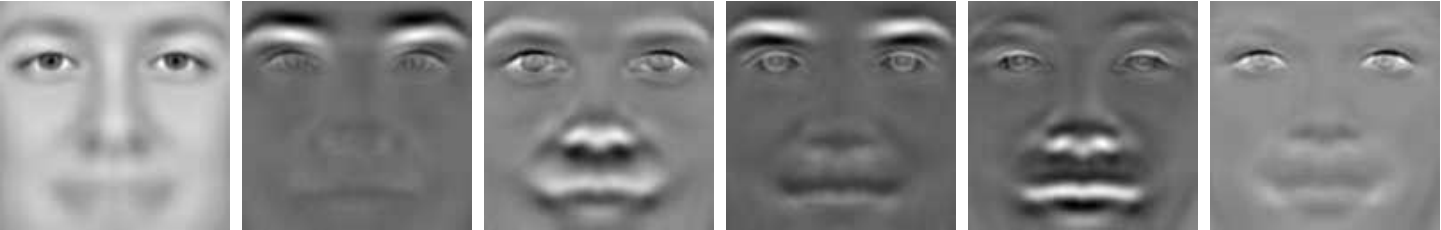
\includegraphics[width=1\linewidth]{img/eigenfaces}
    \caption{Prvých 6 bázových vektorov Eigenfaces, prebraté z\cite[p.~45]{handbookbio}}
    \label{fig:eigenfaces}
\end{figure}

Na obrázku\ref{fig:eigenfaces} vidíme príklad vlastných vektorov vybraných metódou Eigenfaces, na obrázkoch po procese normalizácie.
Metóda PCA je vhodná na reprezentáciu dát, čo neznamená, že je vhodná aj na rozdeľovanie do tried.

\subsubsection{LDA, Fisherfaces}
Matóda LDA\cite{duda2012pattern} je oveľa vhodnejšia k hľadaniu projekcií, ktoré dobre oddeľujú rozdielne triedy.
Táto metóda je založená na hľadaní optimálnych projekčných vektorov, ktoré optimalizujú pomer medzitriednych (within class) a vnútrotriednych (between class) vzdialeností - maximalizuje oddelenie tried
v premietnutom priestore.
Optimálne bázové vektory LDA, môžu byť podľa\cite{handbookbio} definované ako rovnica\eqref{eqn:lda}, kde S\textsubscript{B} značí medzitriednu maticu rozptylu a kde S\textsubscript{W}
vnútrotriednu maticu rozptylu.\\
\indent
\begin{equation}\label{eqn:lda}
W_{LDA} = arg max \frac{|W^T S_B W|}{|W^T S_W W|}
\end{equation}

Zvyčajne pri riešení problematiky rozpoznávania tváre (a vačšine ostatných problémov rozpoznávania vzorov obrázkov) je množstvo tréningových obrázkov menší ako počet pixelov
(dimenzionality dát), čo znamená, že vnútrotriedová matica rozptylu S\textsubscript{W} je singulárna, čo je problémom pre LDA.
Na vyriešenie tohoto problému singulárnej matice sa na najprv vykonáva PCA na redukovanie dimenzionality dát a
až následne sa aplikuje LDA v menej rozmernom podpriestore PCA.
NA základe týchto zmien bolo dosiahnuté zlepšenie výsledkov v porovnaní s tradičnou PCA metódou.
Projekčné vektory, ktorých príklad môžeme vidiet na obrázku\ref{fig:fisherfaces}  Fisherfaces sú tie, ktorú spĺňajú maximalizujú vysledok optimalizačnej funkcie\eqref{eqn:fisher}.

\begin{figure}[H]
    \centering
    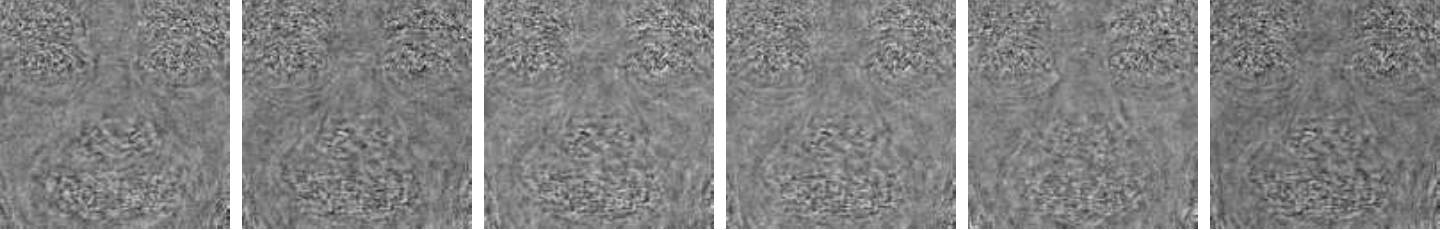
\includegraphics[width=1\linewidth]{img/fisherfaces.png}
    \caption{Prvých 6 bázových vektorov Fisherfaces, prebraté z\cite[p.~46]{handbookbio}}
    \label{fig:fisherfaces}
\end{figure}

\begin{equation}\label{eqn:fisher}
W_{LDA} = arg max \frac{|W^T W_{PCA}^T S_B W_{PCA} W|}{|W^T W_{PCA}^T S_W W_{PCA} W|}
\end{equation}


\subsection{Detekcia tváre}
\subsection{Hľadania bodov tváre}
\subsection{Meranie úspešnosti}
\subsection{Súčasný stav}


%\section{Neurónové siete}
%\subsection{Neurón}
%\subsection{Učenie neuróvej siete}
%\subsection{Konvolučné neurónové siete}
%\subsection{Vrstvy konvolučnej neurónovej siete}
%\subsubsection{Konvolučná vrstva}
%\subsubsection{ReLU vrstva}
%\subsubsection{Pooling vrstva}
%\section{Trénovanie modelu na rozpoznávanie tvárí}
%\subsection{Tensorflow}
%\subsection{Výber datasetu}
%\subsection{Predspracovanie dát}
%\subsection{Facenet}
%\subsection{Klasifikovanie tváre}

%\section{Rospoznávanie tvárí na zariadení Android}
%\subsection{Android OS}
%\subsection{Spracovanie obrazu z kamery}
%\subsection{Detekcia tváre}
%\subsection{Extrahovanie príznakov}
%\subsection{Klasifikácia tváre}
%\subsection{Výkonnostné výsledky}